% !TEX encoding = UTF-8
% !TEX TS-program = pdflatex
% !TEX root = ../tesi.tex

% (3) che risponde alle domande “cosa” e “come”, nel quale racconterai gli elementi essenziali del tuo stage,
% vedendolo come un mini‐progetto a se stante. In questo capitolo illustrerai: (a) il metodo di lavoro con il quale hai
% affrontato lo stage; (b) i problemi progettuali, tecnologici e applicativi che hai affrontati; (c) i risultati che hai
% raggiunto, sia sul piano qualitativo che su quello quantitativo. Il punto (a) comprende la pianificazione, le interazioni
% con il tutor aziendale, le revisioni di progresso, l’uso di diagrammi, di tecniche di analisi e tracciamento dei requisiti,
% l’uso di strumenti di verifica, ecc. Il punto (b), che tratterai nella sequenza di attività che hai svolto (analisi,
% progettazione, programmazione, verifica e validazione), metterà in luce gli aspetti principali, secondo una visione ad
% alto livello. Entrerai in dettaglio solo per aspetti che consideri particolarmente meritevoli di attenzione dal punto di
% vista delle conoscenze acquisite o necessarie. Il punto (c) tratta di copertura di requisiti, di copertura di testing, e di
% quantità di prodotti (linee di codice, numero di documenti, ecc.).


%**************************************************************
\chapter{Resoconto dello stage}
\label{cap:resoconto-stage}
%**************************************************************

\section{Descrizione del progetto}
Parte del progetto che l'azienda mi ha proposto era già stato sviluppato dal team \textit{big data} qualche anno fa.
Il \textit{dataset} da elaborare ed analizzare è infatti parte di un concorso a cui l'azienda aveva partecipato: questa competizione è stata indetta da BNP Paribas Cardif, il polo assicurativo del Gruppo BNP Paribas, e pubblicata su Keggle\footcite{https://www.kaggle.com/}, nota piattaforma in cui è possibile esporre i propri progetti, visualizzare quelli altrui e proporre sfide in ambito \textit{data science} e \textit{machine learning}.

\subsection{Il problema}
In particolare, il problema proposto, "BNP Paribas Cardif Claims Management"\footcite{https://www.kaggle.com/c/bnp-paribas-cardif-claims-management}, consiste nella possibilità di classificare le pratiche assicurative in modo che queste possano essere risolte nel minor tempo possibile. A tal proposito, si chiede di prevedere la categoria di un sinistro sulla base delle caratteristiche disponibili nelle prime fasi del processo assicurativo; le due categorie di richieste di indennizzo, su cui basare la classificazione, corrispondono quindi a:
\begin{itemize}
	\item Quelle per le quali l'approvazione poteva essere accelerata, con conseguente maggiore rapidità nel rimborso e minori pratiche da gestire;
	\item Quelle per le quali erano richieste informazioni supplementari prima dell'approvazione e del rimborso.
\end{itemize}
\clearpage
\begin{figure}[!h] 
	\centering 
	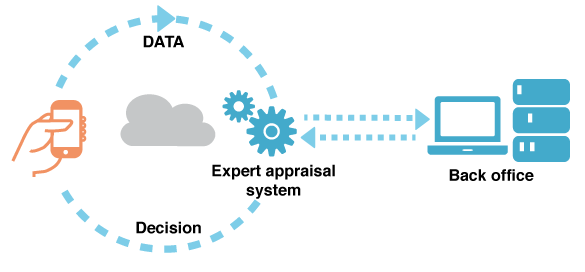
\includegraphics[width=0.7\columnwidth]{kaggle-project}
	\caption{Illustrazione del problema proposto (Fonte: \href{https://goo.gl/AW22at}{https://goo.gl/AW22at})}
\end{figure}
Nella sezione \hyperref[dataset]{Analisi del dataset di interesse} verrà trattata la struttura del \textit{dataset} più nel dettaglio.

%**************************************************************

\section{Studio di Hadoop e dei suoi tools}
Prima di cominciare a lavorare sul \textit{dataset} del progetto, era necessario studiare la teoria, in quanto la prima parte dello stage considerava argomenti a me quasi totalmente sconosciuti.
Autonomamente, ma sempre supervisionato dal tutor aziendale, disponibile a risolvere ogni mio dubbio, ho studiato il materiale necessario per poter eseguire poi al meglio la parte pratica. Oltre a ciò, nel corso della giornata lavorativa, il tutor mi sottoponeva delle esercitazioni da svolgere per consolidare i concetti appresi e risolvere tempestivamente miei eventuali dubbi prima di procedere con gli argomenti successivi.
Essendo \gls{HDFS} e molti dei tool Hadoop eseguibili principalmente tramite \gls{Bash}, come prima cosa mi è stato assegnato lo studio autonomo di alcuni capitoli, selezionati dal tutor, del libro "Learning the bash Shell"\footcite{http://shop.oreilly.com/product/9780596009656.do} per ottenere le basi che mi permettessero di utilizzare i comandi che mi sarebbero serviti in seguito per l'utilizzo dei tool Hadoop.\\
Dopo aver assorbito i concetti, già in parte di mia conoscenza, il tutor mi ha esposto la struttura del \gls{cluster} Hadoop in cui risiedevano i dati e venivano eseguiti i \textit{task}. 
\subsection{Apache Hadoop}
Ogni giorno si generano petabytes di dati che, se processati ed analizzati a dovere possono offrire informazioni con un alto valore strategico per un'azienda. Hadoop nasce dall'esigenza di dover gestire e processare questi dati in modo veloce, tramite una soluzione che sia il più possibile economica e scalabile orizzontalmente: aggiungendo nuovi nodi al cluster, la capacità e le performance di questo infatti aumentano proporzionalmente. Per aumentare ulteriormente le prestazioni e la scalabilità del sistema, Hadoop cerca di elaborare i dati sullo stesso nodo in cui questi risiedono: questo permette di ridurre al minimo la \textit{cross-communication} fra i nodi e la necessità di copiare grandi quantità di dati fra questi, eliminando il rischio di \textit{bottleneck} dovuto dalla velocità di trasmissione dei dati. Per gestire il sistema, Hadoop si basa su:
\begin{itemize}
	\item \gls{HDFS}: per la gestione dei dati persistenti;
	\item YARN: per lo \textit{scheduling} dei processi (\textit{jobs}) e la gestione delle risorse.
\end{itemize}
\begin{figure}[!h]
	\centering 
	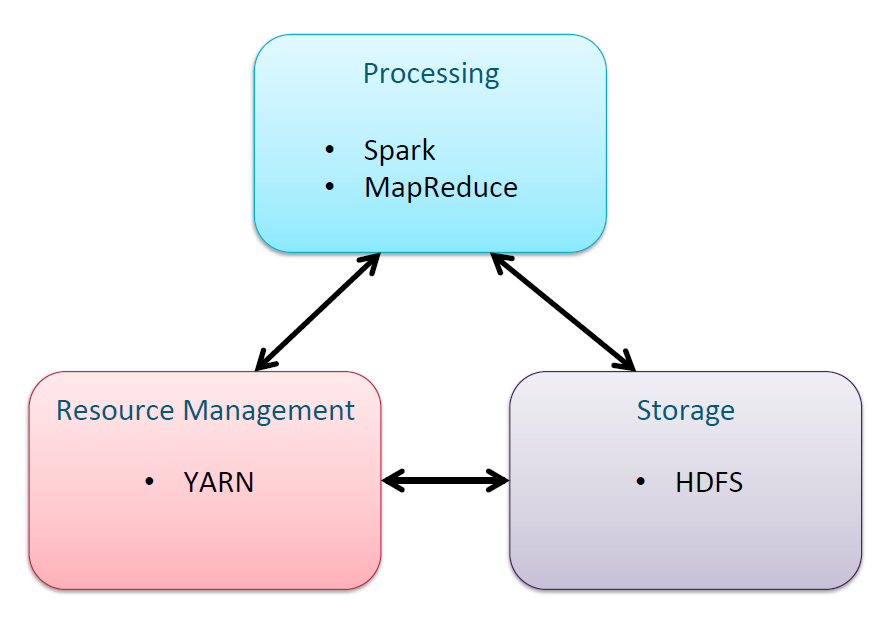
\includegraphics[width=0.7\columnwidth]{hadoop_tools}
	\caption{Attori principali del sistema Hadoop (Fonte: Cloudera - Developer Training for Spark and Hadoop)}
\end{figure}
\subsubsection{HDFS}
Hadoop Distributed File System (HDFS) è un \textit{file system} scritto in Java, basato su Google File System\footcite{https://ai.google/research/pubs/pub51}. \\
Offre performance migliori con un modesto numero di file di grandi dimensioni piuttosto che miliardi di dati frammentati, per questo motivo, anche le operazioni di \textit{read}, sono ottimizzate per la lettura in \textit{streaming} piuttosto che quelle casuali. Inoltre, i file sono tutti \textit{write-once} e quindi non modificabili una volta memorizzati.
In scrittura, infatti, i dati sono suddivisi in blocchi di dimensione fissata e distribuiti tra i nodi una volta caricati in modo ridondante per prevenire la perdita di informazioni nel caso un nodo non fosse più disponibile in seguito.
\begin{figure}[!h]
	\centering
	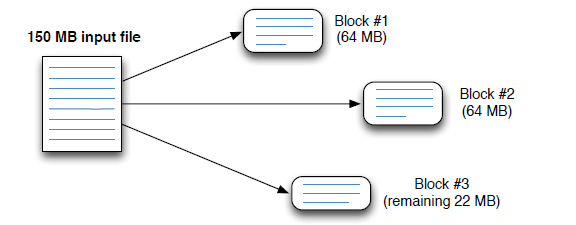
\includegraphics[width=0.8\columnwidth]{data_split}
	\caption{Divisione di un file in blocchi su HDFS (Fonte: Cloudera - Administrator Training for Apache Hadoop)}
\end{figure}
\clearpage
\begin{figure}[!h]
	\centering
	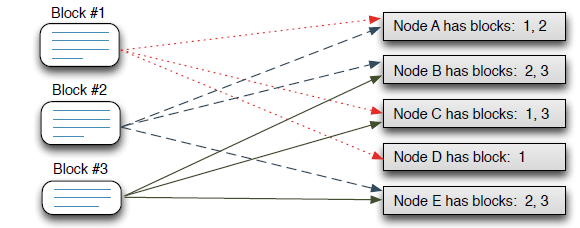
\includegraphics[width=0.8\columnwidth]{data_save}
	\caption{Caricamento dei blocchi nei nodi (Fonte: Cloudera - Administrator Training for Apache Hadoop)}
\end{figure}
Hadoop ha un'architettura di tipo \textit{master-slave}, ovvero in cui il processo \textit{master} ha il controllo su quello \textit{slave}. I nodi, quindi, possono essere di tre tipi:
\begin{itemize}
	\item \textbf{NameNode}: costituisce il \textit{master \gls{daemon}}, quindi gestisce tutti i \textit{metadati}, le informazioni riguardo l'\textit{ownership} e i permessi ad una risorsa, i nomi dei blocchi e la loro locazione. Essendo unico e mantenendo la struttura del \textit{file system}, rappresenta un \gls{single point of failure} in \gls{HDFS};
	\item \textbf{DataNode}: costituisce gli \textit{slave \gls{daemon}}, quindi i nodi che contengono i blocchi di dati veri e propri;
	\item \textbf{Secondary NameNode}: esegue elaborazioni in supporto al NameNode. Non è un nodo di backup ma la funzione principale è quella di memorizzare una copia del file \textit{FsImage} e di modificare il file di log. \textit{FsImage} contiene un'istantanea dei metadati del \textit{file system} HDFS in un certo momento e \textit{EditLog} è il log delle transazioni che contiene record per ogni modifica dei metadati del \textit{file system}. In questo modo, in qualunque momento, è possibile ricostruire il NameNode a partire da \textit{FsImage} e applicando il record delle transazioni \textit{EditLog}.
\end{itemize}
\begin{figure}[!h]
	\centering
	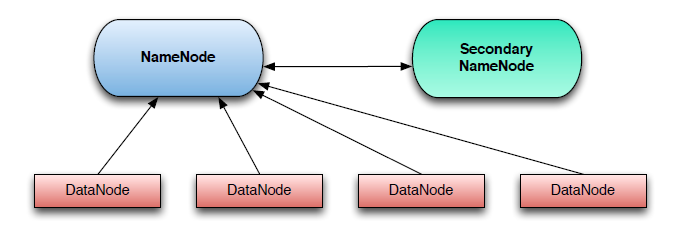
\includegraphics[width=0.8\columnwidth]{hadoop-nodes}
	\caption{Rappresentazione dei nodi in Hadoop (Fonte: Cloudera - Administrator Training for Apache Hadoop)}
\end{figure}
Nei seguenti esempi sono rappresentati semplici operazioni di lettura e scrittura sui nodi HDFS.
La procedura di scrittura di un blocco avviene nel seguente modo:
\begin{enumerate}
	\item Il client si connette al NameNode;
	\item NameNode registra i \textit{metadati} del file e ritorna il nome del blocco e la lista dei DataNodes al client;
	\item Il client si connette al primo DataNode e comincia ad inviare i dati;
	\item A sua volta, il primo DataNode si connette al secondo e invia a sua volta i dati;
	\item Allo stesso modo, il secondo DataNode si connette al terzo;
	\item Ad ogni blocco scritto, al client viene ritornato un \textit{ack packets} dalla \textit{pipeline} di nodi;
	\item Una volta ricevuti tutti gli \textit{ack packets}, il client informa il NameNode del completamento della scrittura.
\end{enumerate} 
\begin{figure}[!h]
	\centering
	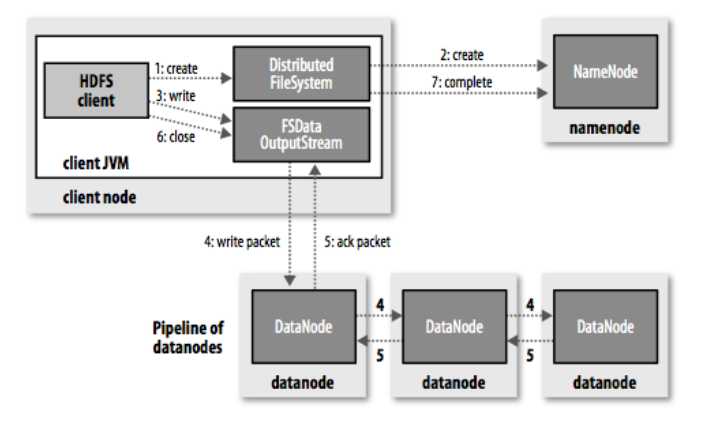
\includegraphics[width=0.65\columnwidth]{hdfs_write}
	\caption{Esempio di scrittura di un file in HDFS (Fonte: Cloudera - Administrator Training for Apache Hadoop)}
\end{figure}
La procedura di lettura di dati avviene nel seguente modo:
\begin{enumerate}
	\item Il client si connette al NameNode;
	\item NameNode ritorna il nome e la locazione dei blocchi del file;
	\item Il client si connette ai DataNodes comunicati e legge i blocchi.
\end{enumerate}
\begin{figure}[!h]
	\centering
	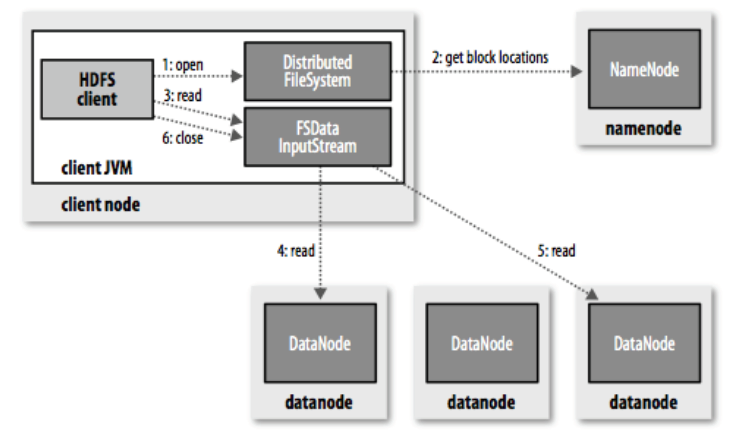
\includegraphics[width=0.65\columnwidth]{hdfs_read}
	\caption{Esempio di lettura di un file in HDFS (Fonte: Cloudera - Administrator Training for Apache Hadoop)}
\end{figure}

\subsubsection{YARN}
YARN (\textit{Yet Another Resource Negotiator}) è il manager delle risorse di Hadoop. I principali attori del sistema sono:
\begin{itemize}
	\item \textbf{ResourceManager}: uno per \gls{cluster}, e costituisce il \textit{master \gls{daemon}}; inizializza le applicazioni e ne pianifica l'utilizzo delle risorse sugli \textit{slave nodes}. È costituito da due componenti principali: uno \textbf{\textit{scheduler}} responsabile per l'allocazione delle risorse delle applicazioni al loro avvio ed un \textbf{\textit{application manager}} che gestisce le applicazioni già in esecuzione sul \textit{cluster};
	\item \textbf{NodeManager}: uno per \textit{slave nodes} e costituisce lo \textit{slave \gls{daemon}}; avvia i processi delle applicazioni e gestisce le risorse sul singolo \textit{slave node};
	\item \textbf{JobHistoryServer}: uno per \gls{cluster}, archivia i log ed i \textit{metadata} dei \textit{jobs} terminati;
	\item \textbf{ApplicationManager}: uno per applicazione, negozia le risorse con il ResourceManager e lavora con il NodeManager; gestisce l'intera vita dell'applicazione, dalla sua inizializzazione al suo termine. 
\end{itemize}
\begin{figure}[!h]
	\centering
	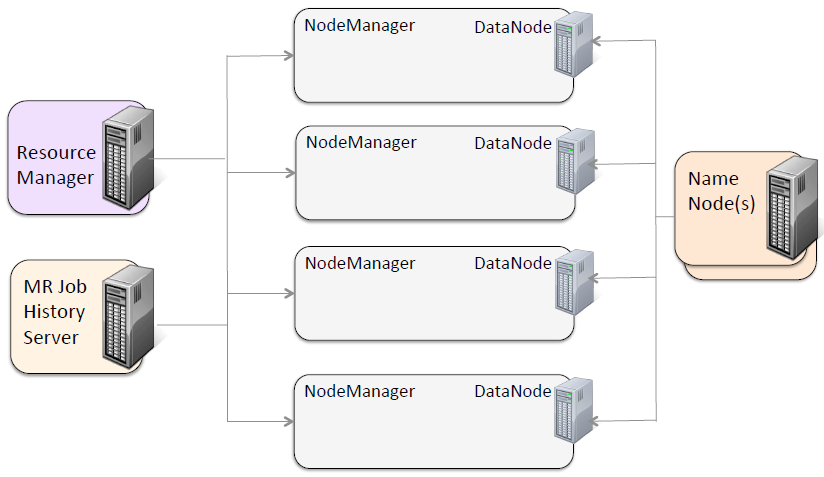
\includegraphics[width=0.8\columnwidth]{yarn_architecture}
	\caption{Struttura di un cluster che utilizza YARN (Fonte: Cloudera - Administrator Training for Apache Hadoop)}
\end{figure}
YARN, per avviare un'applicazione sul \gls{cluster}, si comporta nel modo seguente:
\begin{enumerate}
	\item Il client richiede di eseguire un \textit{job} al ResourceManager che inizializza un \textit{container}, ovvero un numero finito di risorse di un nodo, e avvia l'ApplicationManager sul NodeManager;
	\item L'ApplicationManager richiede le risorse necessarie per eseguire tutti i \textit{tasks} al ResourceManager;
	\item Il ResourceManager alloca nuovi \textit{containers} su altri nodi del \gls{cluster} e comunica all'ApplicationManager la loro locazione;
	\item L'ApplicationManager esegue i \textit{tasks} nei \textit{containers} allocati precedentemente;
	\item Una volta completato il \textit{job}, l'ApplicationManager segnala al ResourceManager la conclusione del processo.
\end{enumerate} 
\begin{figure}[!h]
	\centering
	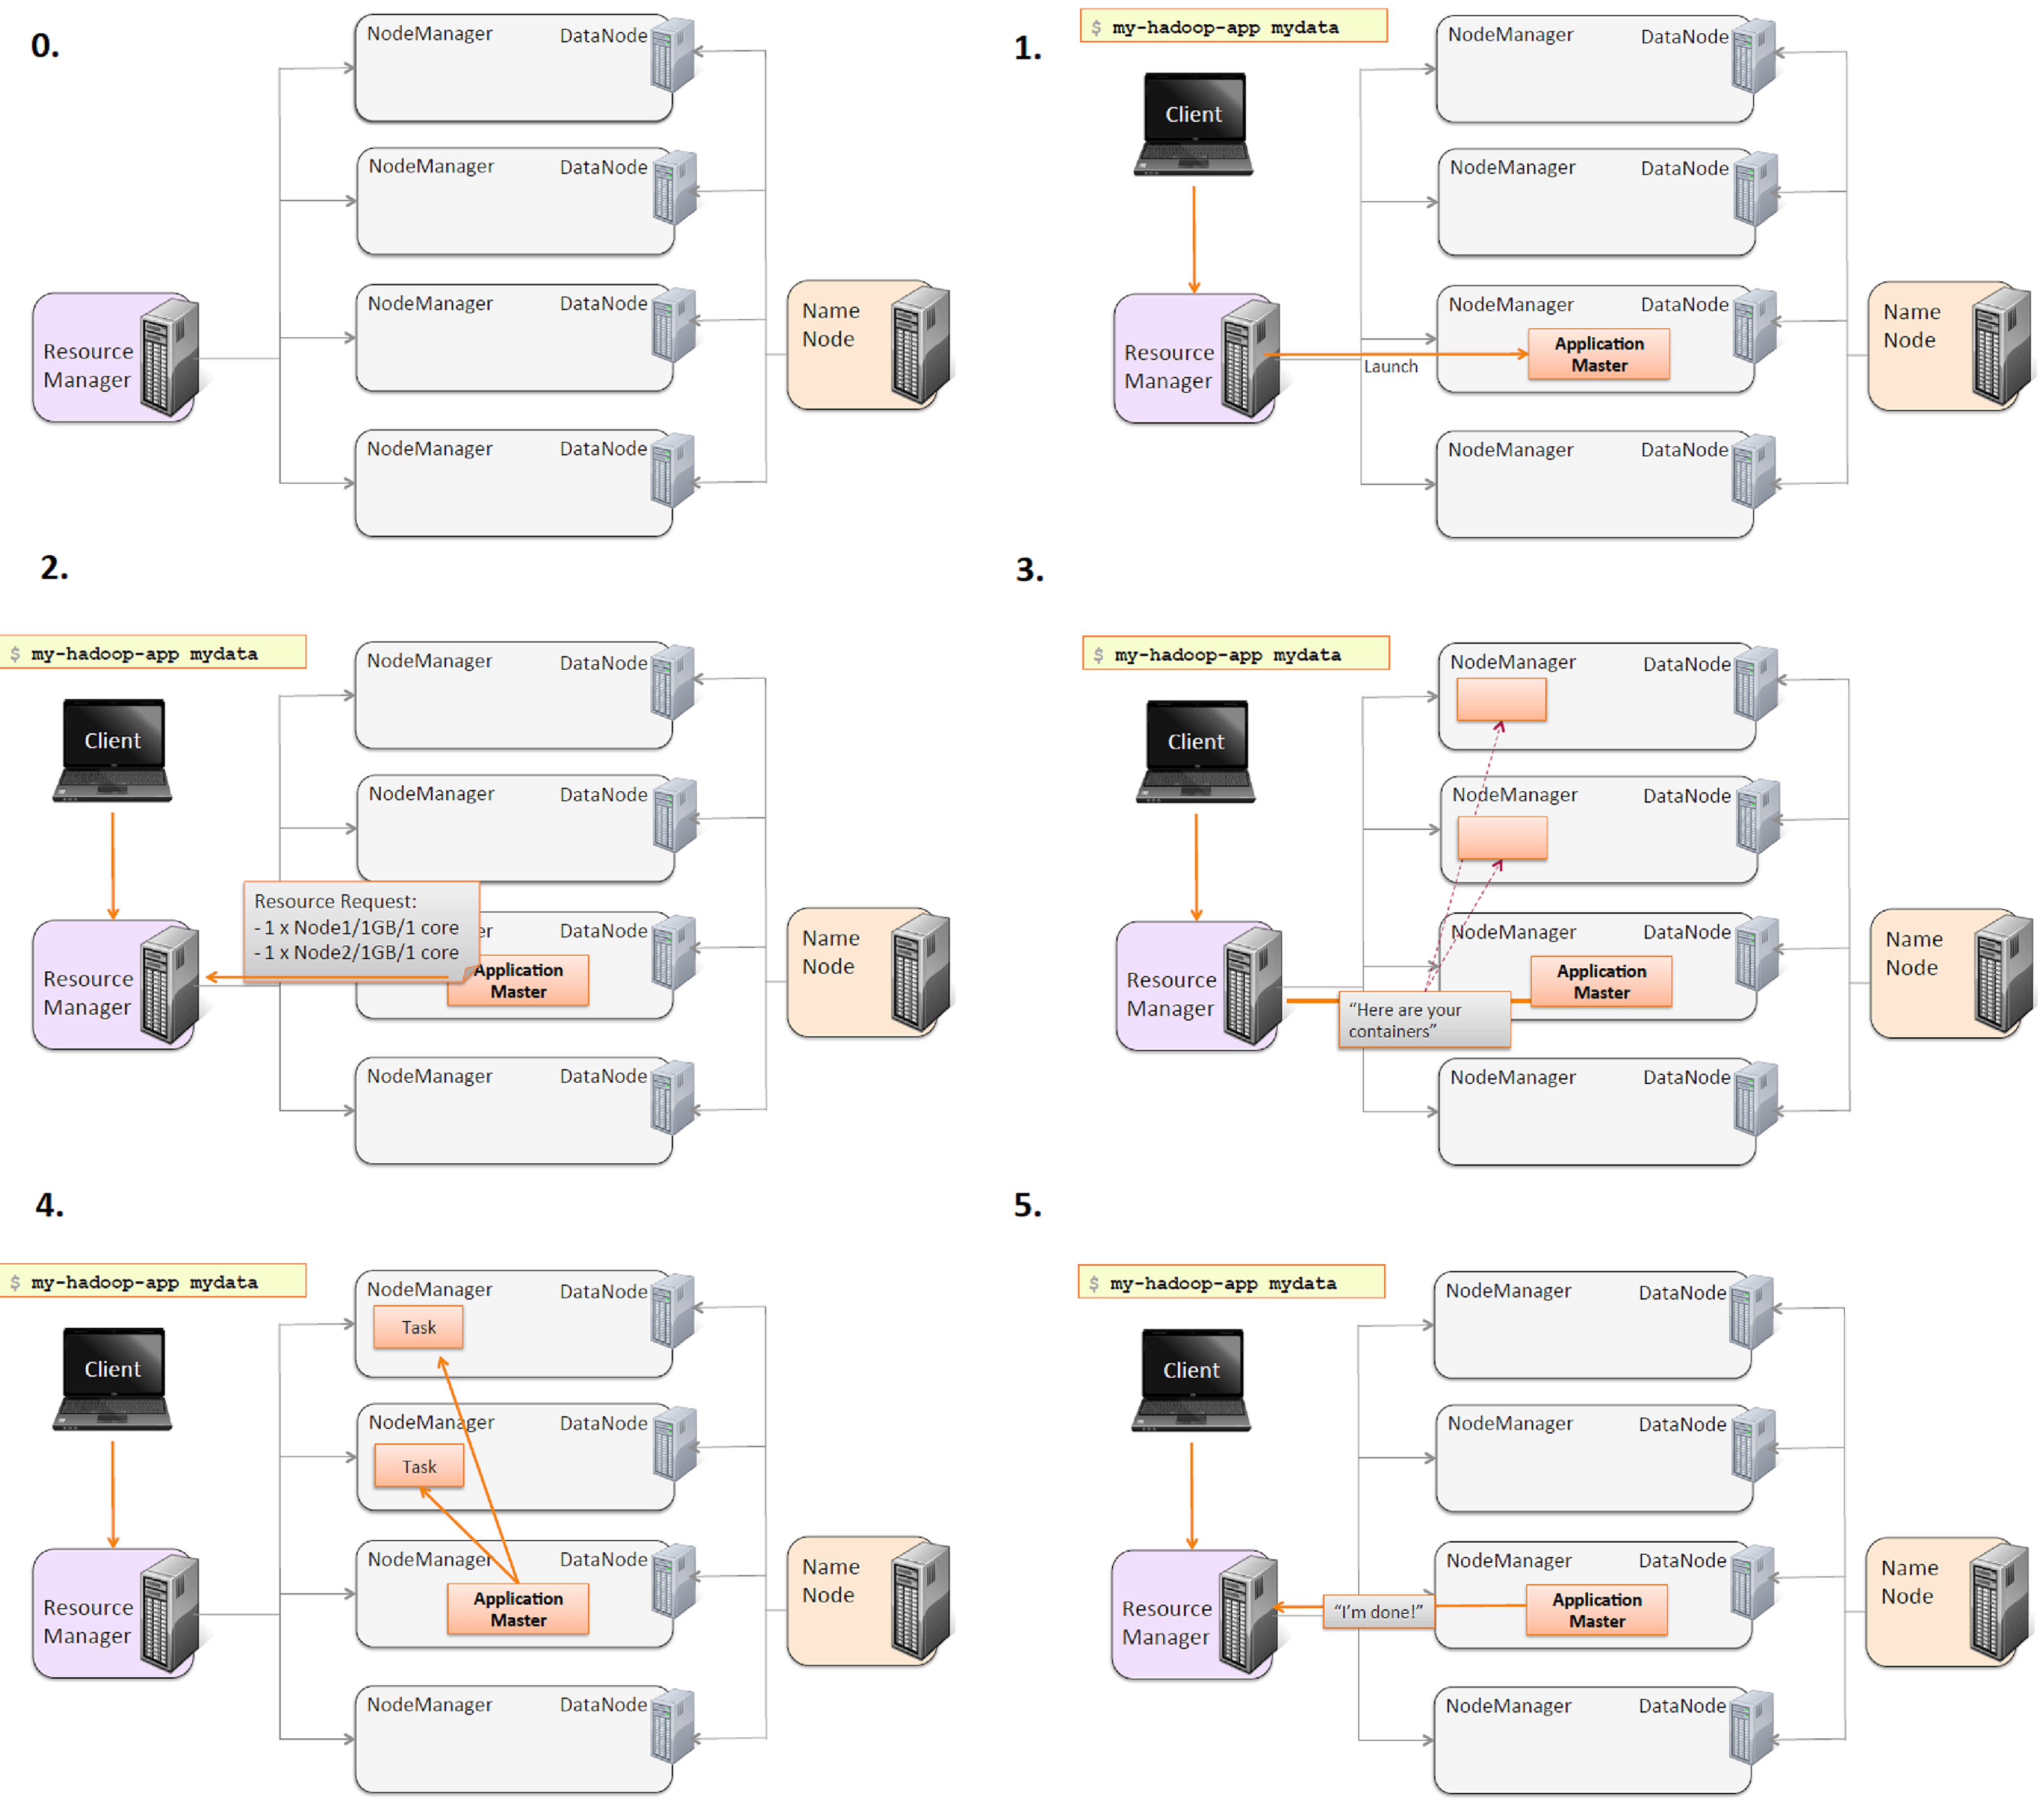
\includegraphics[width=1.2\columnwidth]{yarn_application}
	\caption{Sequenza avvio applicazione di YARN}
\end{figure}
\newpage
\subsection{Apache Hive, Apache Spark e Cloudera Impala}
\subsubsection{Apache Hive}
Originariamente sviluppato da Facebook per facilitare l'interrogazioni di \textit{dataset} su Hadoop, fornisce un metodo per effettuare \textit{query} in HDFS utilizzando un linguaggio simile ad SQL chiamato HiveQL. 
Le \textit{query} sono poi convertite da Hive in \textit{jobs} che vengono eseguiti da YARN. A causa di questa conversione, i risultati di una \textit{query} sono lenti, infatti ottenere un risultato può richiedere anche minuti se non ore. Inoltre, come detto in precedenza, in HDFS non è possibile modificare i dati, e quindi le operazioni di UPDATE e DELETE, tipiche di SQL, non sono supportate.
Hive interpreta tutti i file di una directory HDFS come contenuti di una tabella e salva le informazioni su come le righe e le colonne della tabella sono delimitate in una locazione, che può essere sulla macchina locale dell'utente o condivisa fra più utenti, chiamata \textbf{Hive Metastore}.
Nel caso Hive Metastore sia condiviso, il client si connette ad un'altro attore, chiamato \textbf{Hive Metastore Service} utilizzando le \gls{api} di Apache Thrift\footcite{https://thrift.apache.org/}. A sua volta, questo si connette al Metastore attraverso le Java JDBC.
\begin{figure}[!h]
	\centering
	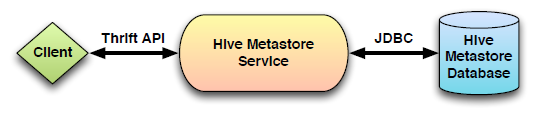
\includegraphics[width=0.8\columnwidth]{hive-metastore}
	\caption{Rappresentazione delle connessioni ad Hive Metastore (Fonte: Cloudera - Administrator Training for Apache Hadoop)}
\end{figure}

%**************************************************************
\section{Analisi del dataset di interesse} \label{dataset}

%**************************************************************

\section{Progettazione e sviluppo della web app}
